\documentclass[twoside]{book}

% Packages required by doxygen
\usepackage{calc}
\usepackage{doxygen}
\usepackage{graphicx}
\usepackage[utf8]{inputenc}
\usepackage{makeidx}
\usepackage{multicol}
\usepackage{multirow}
\PassOptionsToPackage{warn}{textcomp}
\usepackage{textcomp}
\usepackage[nointegrals]{wasysym}
\usepackage[table]{xcolor}

% Font selection
\usepackage[T1]{fontenc}
\usepackage{mathptmx}
\usepackage[scaled=.90]{helvet}
\usepackage{courier}
\usepackage{amssymb}
\usepackage{sectsty}
\renewcommand{\familydefault}{\sfdefault}
\allsectionsfont{%
  \fontseries{bc}\selectfont%
  \color{darkgray}%
}
\renewcommand{\DoxyLabelFont}{%
  \fontseries{bc}\selectfont%
  \color{darkgray}%
}
\newcommand{\+}{\discretionary{\mbox{\scriptsize$\hookleftarrow$}}{}{}}

% Page & text layout
\usepackage{geometry}
\geometry{%
  a4paper,%
  top=2.5cm,%
  bottom=2.5cm,%
  left=2.5cm,%
  right=2.5cm%
}
\tolerance=750
\hfuzz=15pt
\hbadness=750
\setlength{\emergencystretch}{15pt}
\setlength{\parindent}{0cm}
\setlength{\parskip}{0.2cm}
\makeatletter
\renewcommand{\paragraph}{%
  \@startsection{paragraph}{4}{0ex}{-1.0ex}{1.0ex}{%
    \normalfont\normalsize\bfseries\SS@parafont%
  }%
}
\renewcommand{\subparagraph}{%
  \@startsection{subparagraph}{5}{0ex}{-1.0ex}{1.0ex}{%
    \normalfont\normalsize\bfseries\SS@subparafont%
  }%
}
\makeatother

% Headers & footers
\usepackage{fancyhdr}
\pagestyle{fancyplain}
\fancyhead[LE]{\fancyplain{}{\bfseries\thepage}}
\fancyhead[CE]{\fancyplain{}{}}
\fancyhead[RE]{\fancyplain{}{\bfseries\leftmark}}
\fancyhead[LO]{\fancyplain{}{\bfseries\rightmark}}
\fancyhead[CO]{\fancyplain{}{}}
\fancyhead[RO]{\fancyplain{}{\bfseries\thepage}}
\fancyfoot[LE]{\fancyplain{}{}}
\fancyfoot[CE]{\fancyplain{}{}}
\fancyfoot[RE]{\fancyplain{}{\bfseries\scriptsize Generated on Thu Feb 20 2014 14\+:47\+:29 for L\+E\+D\+Cube by Doxygen }}
\fancyfoot[LO]{\fancyplain{}{\bfseries\scriptsize Generated on Thu Feb 20 2014 14\+:47\+:29 for L\+E\+D\+Cube by Doxygen }}
\fancyfoot[CO]{\fancyplain{}{}}
\fancyfoot[RO]{\fancyplain{}{}}
\renewcommand{\footrulewidth}{0.4pt}
\renewcommand{\chaptermark}[1]{%
  \markboth{#1}{}%
}
\renewcommand{\sectionmark}[1]{%
  \markright{\thesection\ #1}%
}

% Indices & bibliography
\usepackage{natbib}
\usepackage[titles]{tocloft}
\setcounter{tocdepth}{3}
\setcounter{secnumdepth}{5}
\makeindex

% Hyperlinks (required, but should be loaded last)
\usepackage{ifpdf}
\ifpdf
  \usepackage[pdftex,pagebackref=true]{hyperref}
\else
  \usepackage[ps2pdf,pagebackref=true]{hyperref}
\fi
\hypersetup{%
  colorlinks=true,%
  linkcolor=blue,%
  citecolor=blue,%
  unicode%
}

% Custom commands
\newcommand{\clearemptydoublepage}{%
  \newpage{\pagestyle{empty}\cleardoublepage}%
}


%===== C O N T E N T S =====

\begin{document}

% Titlepage & ToC
\hypersetup{pageanchor=false,
             bookmarks=true,
             bookmarksnumbered=true,
             pdfencoding=unicode
            }
\pagenumbering{roman}
\begin{titlepage}
\vspace*{7cm}
\begin{center}%
{\Large L\+E\+D\+Cube \\[1ex]\large 0.\+0.\+1 }\\
\vspace*{1cm}
{\large Generated by Doxygen 1.8.6}\\
\vspace*{0.5cm}
{\small Thu Feb 20 2014 14:47:29}\\
\end{center}
\end{titlepage}
\clearemptydoublepage
\tableofcontents
\clearemptydoublepage
\pagenumbering{arabic}
\hypersetup{pageanchor=true}

%--- Begin generated contents ---
\chapter{Hierarchical Index}
\section{Class Hierarchy}
This inheritance list is sorted roughly, but not completely, alphabetically\+:\begin{DoxyCompactList}
\item Q\+G\+L\+Widget\begin{DoxyCompactList}
\item \contentsline{section}{Matrix\+Widget}{\pageref{class_matrix_widget}}{}
\end{DoxyCompactList}
\item Q\+Main\+Window\begin{DoxyCompactList}
\item \contentsline{section}{Window}{\pageref{class_window}}{}
\end{DoxyCompactList}
\end{DoxyCompactList}

\chapter{Data Structure Index}
\section{Data Structures}
Here are the data structures with brief descriptions\+:\begin{DoxyCompactList}
\item\contentsline{section}{\hyperlink{class_matrix_widget}{Matrix\+Widget} \\*L\+E\+D\+Matrix Widget }{\pageref{class_matrix_widget}}{}
\item\contentsline{section}{\hyperlink{class_window}{Window} \\*The main window of the application }{\pageref{class_window}}{}
\end{DoxyCompactList}

\chapter{Data Structure Documentation}
\hypertarget{class_matrix_widget}{\section{Matrix\+Widget Class Reference}
\label{class_matrix_widget}\index{Matrix\+Widget@{Matrix\+Widget}}
}


L\+E\+D\+Matrix Widget.  




{\ttfamily \#include $<$matrixwidget.\+h$>$}

Inheritance diagram for Matrix\+Widget\+:\begin{figure}[H]
\begin{center}
\leavevmode
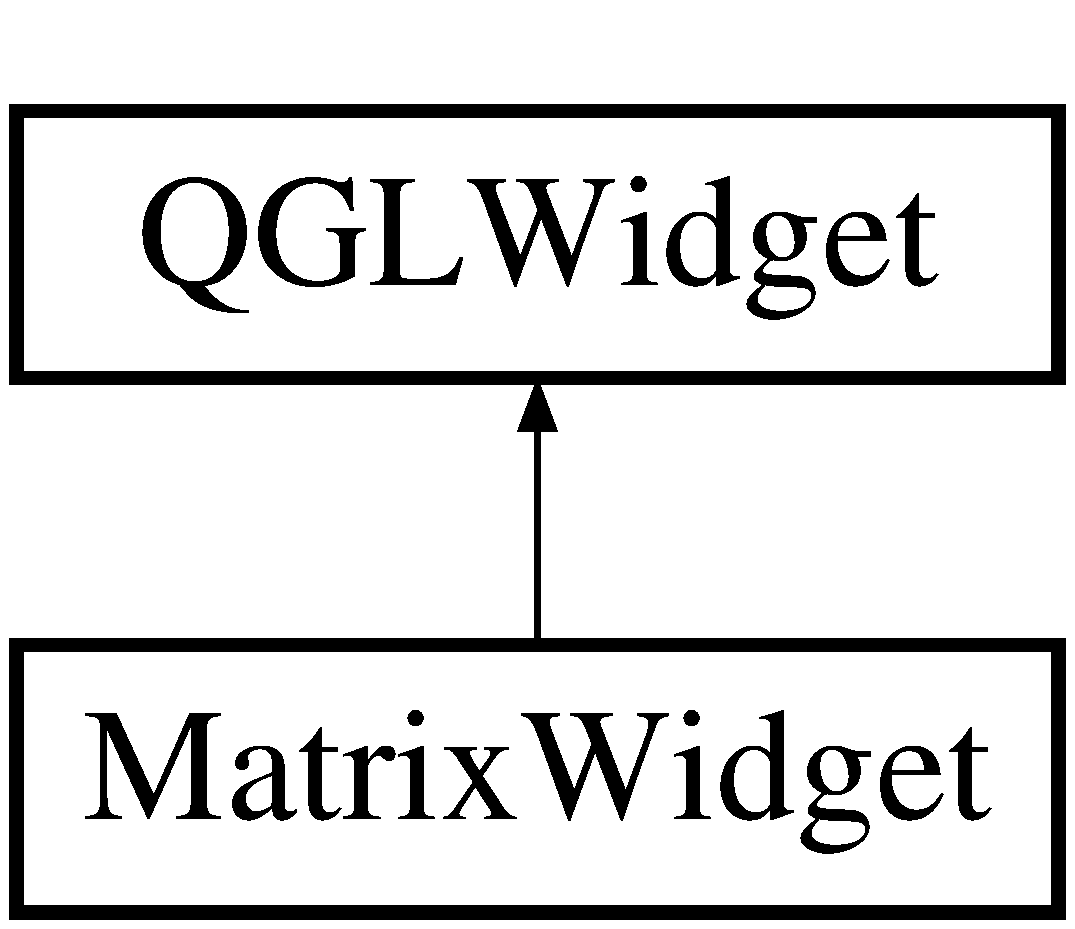
\includegraphics[height=2.000000cm]{class_matrix_widget}
\end{center}
\end{figure}
\subsection*{Public Slots}
\begin{DoxyCompactItemize}
\item 
\hypertarget{class_matrix_widget_a5bad5bfa5cd3c567c0becbd2b1418214}{void {\bfseries set\+X\+Rotation} (int angle)}\label{class_matrix_widget_a5bad5bfa5cd3c567c0becbd2b1418214}

\item 
\hypertarget{class_matrix_widget_a5079e971ba09d29a296e1794a83a962f}{void {\bfseries set\+Y\+Rotation} (int angle)}\label{class_matrix_widget_a5079e971ba09d29a296e1794a83a962f}

\item 
\hypertarget{class_matrix_widget_a874af5a3121de026d6d6d1d1e6dcbd3a}{void {\bfseries set\+Z\+Rotation} (int angle)}\label{class_matrix_widget_a874af5a3121de026d6d6d1d1e6dcbd3a}

\item 
\hypertarget{class_matrix_widget_a281f2b0b02858ce8f02af9acdb1101a6}{void {\bfseries set\+Zoom} (int zoom)}\label{class_matrix_widget_a281f2b0b02858ce8f02af9acdb1101a6}

\item 
\hypertarget{class_matrix_widget_a556d5f41bc0558be7da8d9b9e88beda4}{void {\bfseries set\+X\+Size} (int size)}\label{class_matrix_widget_a556d5f41bc0558be7da8d9b9e88beda4}

\item 
\hypertarget{class_matrix_widget_a0135c4b640238be89682b030b9f1087c}{void {\bfseries set\+Y\+Size} (int size)}\label{class_matrix_widget_a0135c4b640238be89682b030b9f1087c}

\item 
\hypertarget{class_matrix_widget_a6a1daa02d97ff9207c1fa8b0d22033d7}{void {\bfseries set\+Z\+Size} (int size)}\label{class_matrix_widget_a6a1daa02d97ff9207c1fa8b0d22033d7}

\end{DoxyCompactItemize}
\subsection*{Signals}
\begin{DoxyCompactItemize}
\item 
\hypertarget{class_matrix_widget_a8ca3c8b5f4bee3639e3796888467bd4e}{void {\bfseries x\+Rotation\+Changed} (int angle)}\label{class_matrix_widget_a8ca3c8b5f4bee3639e3796888467bd4e}

\item 
\hypertarget{class_matrix_widget_a6ccdf79103c98aaebb433ea80640533b}{void {\bfseries y\+Rotation\+Changed} (int angle)}\label{class_matrix_widget_a6ccdf79103c98aaebb433ea80640533b}

\item 
\hypertarget{class_matrix_widget_a10801025feb3fa29eed36d30c0de1d6e}{void {\bfseries z\+Rotation\+Changed} (int angle)}\label{class_matrix_widget_a10801025feb3fa29eed36d30c0de1d6e}

\end{DoxyCompactItemize}
\subsection*{Public Member Functions}
\begin{DoxyCompactItemize}
\item 
\hypertarget{class_matrix_widget_a9ff859d14c9b69480e4d57ebd51905e8}{{\bfseries Matrix\+Widget} (Q\+Widget $\ast$parent=0)}\label{class_matrix_widget_a9ff859d14c9b69480e4d57ebd51905e8}

\end{DoxyCompactItemize}
\subsection*{Protected Member Functions}
\begin{DoxyCompactItemize}
\item 
\hypertarget{class_matrix_widget_a11dff2ead5ef6f4f09528cd33fc8c1ff}{void {\bfseries draw\+Cube} (int x, int y, int z)}\label{class_matrix_widget_a11dff2ead5ef6f4f09528cd33fc8c1ff}

\item 
\hypertarget{class_matrix_widget_aaf91ee7b7b9d6f2497b6b1f982bf2585}{void {\bfseries initialize\+G\+L} ()}\label{class_matrix_widget_aaf91ee7b7b9d6f2497b6b1f982bf2585}

\item 
\hypertarget{class_matrix_widget_a72e5ef9c915cfe97da589fcdd87c89bb}{void {\bfseries paint\+G\+L} ()}\label{class_matrix_widget_a72e5ef9c915cfe97da589fcdd87c89bb}

\item 
\hypertarget{class_matrix_widget_afcf4d2da8449cfe3681913183f52671f}{void {\bfseries resize\+G\+L} (int width, int height)}\label{class_matrix_widget_afcf4d2da8449cfe3681913183f52671f}

\item 
\hypertarget{class_matrix_widget_aa4566c137db014cf83f5fe309b4d125f}{void {\bfseries mouse\+Press\+Event} (Q\+Mouse\+Event $\ast$event)}\label{class_matrix_widget_aa4566c137db014cf83f5fe309b4d125f}

\item 
\hypertarget{class_matrix_widget_a654d8f69e0ec87c19bdc11646b4887ff}{void {\bfseries mouse\+Move\+Event} (Q\+Mouse\+Event $\ast$event)}\label{class_matrix_widget_a654d8f69e0ec87c19bdc11646b4887ff}

\item 
\hypertarget{class_matrix_widget_a767e048f16f9c6cac59ab5ba68a4de1f}{float {\bfseries x\+Coords} (int index)}\label{class_matrix_widget_a767e048f16f9c6cac59ab5ba68a4de1f}

\item 
\hypertarget{class_matrix_widget_a84a270b0c96df951e8580df88381a7e4}{float {\bfseries y\+Coords} (int index)}\label{class_matrix_widget_a84a270b0c96df951e8580df88381a7e4}

\item 
\hypertarget{class_matrix_widget_a8f975ec0baa66415ad61be2166c16c7c}{float {\bfseries z\+Coords} (int index)}\label{class_matrix_widget_a8f975ec0baa66415ad61be2166c16c7c}

\item 
\hypertarget{class_matrix_widget_a1b5864e74270c9ec65366f7a2874b90f}{Q\+Size {\bfseries minimum\+Size\+Hint} () const }\label{class_matrix_widget_a1b5864e74270c9ec65366f7a2874b90f}

\item 
\hypertarget{class_matrix_widget_a251e1b90629607fb142d969abbf1ae08}{Q\+Size {\bfseries size\+Hint} () const }\label{class_matrix_widget_a251e1b90629607fb142d969abbf1ae08}

\item 
\hypertarget{class_matrix_widget_a80dca609ac4fe46d5bb1b40f20d04c61}{void {\bfseries calc\+Cube\+Size} ()}\label{class_matrix_widget_a80dca609ac4fe46d5bb1b40f20d04c61}

\item 
\hypertarget{class_matrix_widget_a07494e16ed8ac47a925070fd80b567a6}{bool {\bfseries is\+On} (int x, int y, int z)}\label{class_matrix_widget_a07494e16ed8ac47a925070fd80b567a6}

\item 
\hypertarget{class_matrix_widget_a5fcea4d4e96684f5d84c55bd1d6dea4b}{void {\bfseries perspective} (G\+Ldouble fovy, G\+Ldouble aspect, G\+Ldouble z\+Near, G\+Ldouble z\+Far)}\label{class_matrix_widget_a5fcea4d4e96684f5d84c55bd1d6dea4b}

\end{DoxyCompactItemize}


\subsection{Detailed Description}
L\+E\+D\+Matrix Widget. 

Extension of Q\+G\+L\+Widget on which the actual led matrix is displayed. 

The documentation for this class was generated from the following files\+:\begin{DoxyCompactItemize}
\item 
matrixwidget.\+h\item 
matrixwidget.\+cpp\item 
moc\+\_\+matrixwidget.\+cpp\end{DoxyCompactItemize}

\hypertarget{class_window}{\section{Window Class Reference}
\label{class_window}\index{Window@{Window}}
}


The main window of the application.  




{\ttfamily \#include $<$window.\+h$>$}

Inheritance diagram for Window\+:\begin{figure}[H]
\begin{center}
\leavevmode
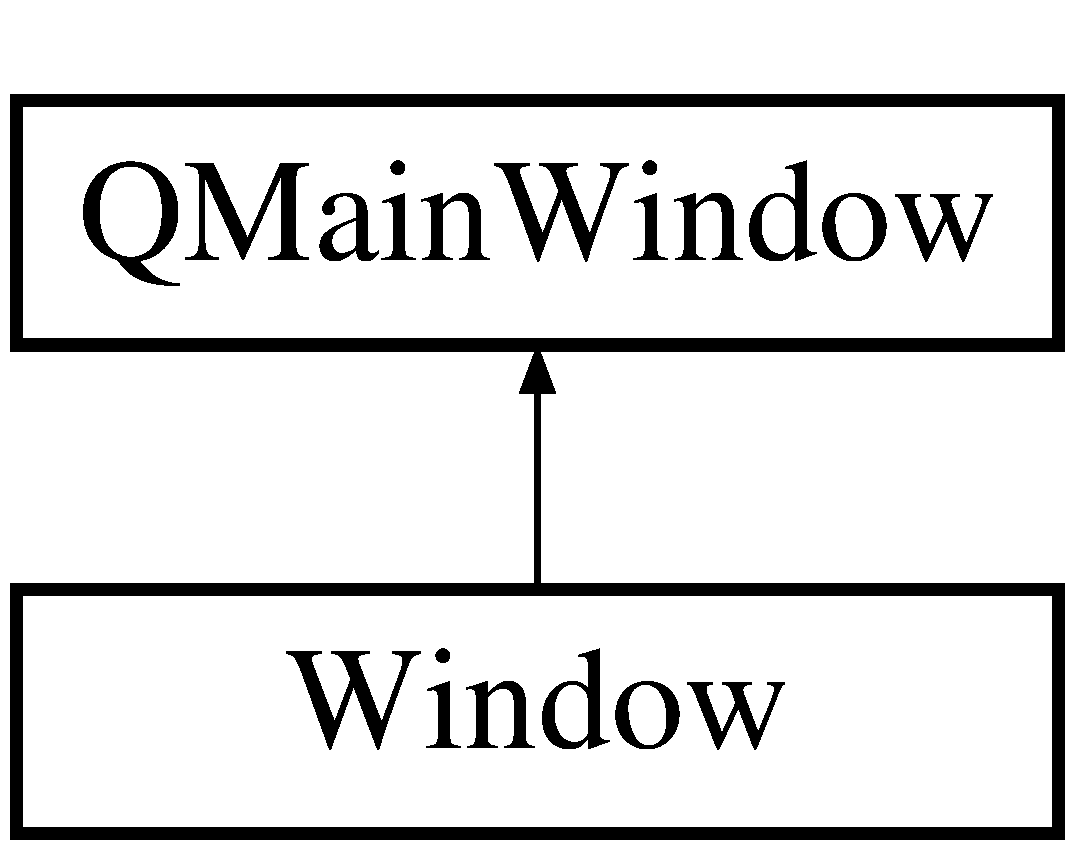
\includegraphics[height=2.000000cm]{class_window}
\end{center}
\end{figure}
\subsection*{Protected Member Functions}
\begin{DoxyCompactItemize}
\item 
\hypertarget{class_window_a52322a90bc51afcd17b90a152d64f36a}{void {\bfseries key\+Press\+Event} (Q\+Key\+Event $\ast$event)}\label{class_window_a52322a90bc51afcd17b90a152d64f36a}

\end{DoxyCompactItemize}


\subsection{Detailed Description}
The main window of the application. 

Is the container for the L\+E\+D\+Matrix widget and the various sliders, spinboxes, etc... 

The documentation for this class was generated from the following files\+:\begin{DoxyCompactItemize}
\item 
window.\+h\item 
window.\+cpp\end{DoxyCompactItemize}

%--- End generated contents ---

% Index
\newpage
\phantomsection
\addcontentsline{toc}{chapter}{Index}
\printindex

\end{document}
